\documentclass[useAMS,usenatbib,usegraphicx,referee]{biom}\usepackage[]{graphicx}\usepackage[]{color}
%% maxwidth is the original width if it is less than linewidth
%% otherwise use linewidth (to make sure the graphics do not exceed the margin)
\makeatletter
\def\maxwidth{ %
  \ifdim\Gin@nat@width>\linewidth
    \linewidth
  \else
    \Gin@nat@width
  \fi
}
\makeatother

\definecolor{fgcolor}{rgb}{0.345, 0.345, 0.345}
\newcommand{\hlnum}[1]{\textcolor[rgb]{0.686,0.059,0.569}{#1}}%
\newcommand{\hlstr}[1]{\textcolor[rgb]{0.192,0.494,0.8}{#1}}%
\newcommand{\hlcom}[1]{\textcolor[rgb]{0.678,0.584,0.686}{\textit{#1}}}%
\newcommand{\hlopt}[1]{\textcolor[rgb]{0,0,0}{#1}}%
\newcommand{\hlstd}[1]{\textcolor[rgb]{0.345,0.345,0.345}{#1}}%
\newcommand{\hlkwa}[1]{\textcolor[rgb]{0.161,0.373,0.58}{\textbf{#1}}}%
\newcommand{\hlkwb}[1]{\textcolor[rgb]{0.69,0.353,0.396}{#1}}%
\newcommand{\hlkwc}[1]{\textcolor[rgb]{0.333,0.667,0.333}{#1}}%
\newcommand{\hlkwd}[1]{\textcolor[rgb]{0.737,0.353,0.396}{\textbf{#1}}}%

\usepackage{framed}
\makeatletter
\newenvironment{kframe}{%
 \def\at@end@of@kframe{}%
 \ifinner\ifhmode%
  \def\at@end@of@kframe{\end{minipage}}%
  \begin{minipage}{\columnwidth}%
 \fi\fi%
 \def\FrameCommand##1{\hskip\@totalleftmargin \hskip-\fboxsep
 \colorbox{shadecolor}{##1}\hskip-\fboxsep
     % There is no \\@totalrightmargin, so:
     \hskip-\linewidth \hskip-\@totalleftmargin \hskip\columnwidth}%
 \MakeFramed {\advance\hsize-\width
   \@totalleftmargin\z@ \linewidth\hsize
   \@setminipage}}%
 {\par\unskip\endMakeFramed%
 \at@end@of@kframe}
\makeatother

\definecolor{shadecolor}{rgb}{.97, .97, .97}
\definecolor{messagecolor}{rgb}{0, 0, 0}
\definecolor{warningcolor}{rgb}{1, 0, 1}
\definecolor{errorcolor}{rgb}{1, 0, 0}
\newenvironment{knitrout}{}{} % an empty environment to be redefined in TeX

\usepackage{alltt}

%  If your system does not have the AMS fonts version 2.0 installed, then
%  remove the useAMS option.
%
%  useAMS allows you to obtain upright Greek characters.
%  e.g. \umu, \upi etc.  See the section on "Upright Greek characters" in
%  this guide for further information.
%
%  If you are using AMS 2.0 fonts, bold math letters/symbols are available
%  at a larger range of sizes for NFSS release 1 and 2 (using \boldmath or
%  preferably \bmath).
% 
%  Other options are described in the user guide. Here are a few:
% 
%  -  If you use Patrick Daly's natbib  to cross-reference your 
%     bibliography entries, use the usenatbib option
%
%  -  If you use \includegraphics (graphicx package) for importing graphics
%     into your figures, use the usegraphicx option
% 
%  If you wish to typeset the paper in Times font (if you do not have the
%  PostScript Type 1 Computer Modern fonts you will need to do this to get
%  smoother fonts in a PDF file) then uncomment the next line
%  \usepackage{Times}
\usepackage{amsmath,amsfonts,framed,booktabs,bm,mathrsfs}
% \usepackage[boxed]{algorithm2e}

%%%%% PLACE YOUR OWN MACROS HERE %%%%%
\newcommand{\diag}{\operatorname{diag}}
\newcommand{\E}{\operatorname{E}}
\newcommand{\var}{\operatorname{Var}}
\newcommand{\cov}{\operatorname{Cov}}
\newcommand{\se}{\operatorname{se}}
\newcommand{\trans}{\ensuremath{^\prime}}
\newcommand{\boot}{\star} 
\newcommand{\code}[1]{\texttt{#1}}
\newcommand{\proglang}[1]{\textsf{#1}}
\newcommand{\pkg}[1]{{\fontseries{b}\selectfont #1}}
\newcommand{\X}{\ensuremath{\bm{X}}}
\newcommand{\Z}{\ensuremath{\bm{Z}}}
\newcommand{\newln}{\\&\quad\quad\quad\quad{}}

%  The rotating package allows you to have tables displayed in landscape
%  mode.  The rotating package is NOT included in this distribution, but
%  can be obtained from the CTAN archive.  USE OF LANDSCAPE TABLES IS
%  STRONGLY DISCOURAGED -- create landscape tables only as a last resort if
%  you see no other way to display the information.  If you do do this,
%  then you need the following command.

%\usepackage[figuresright]{rotating}

%%%%%%%%%%%%%%%%%%%%%%%%%%%%%%%%%%%%%%%%%%%%%%%%%%%%%%%%%%%%%%%%%%%%%




%%%%%%%%%%%%%%%%%%%%%%%%%%%%%%%%%%%%%%%%%%%%%%%%%%%%%%%%%%%%%%%%%%%%%

%  Here, place your title and author information.  Note that in 
%  use of the \author command, you create your own footnotes.  Follow
%  the examples below in creating your author and affiliation information.
%  Also consult a recent issue of the journal for examples of formatting.

\title[Linear Calibration with Grouped Data]{Linear Calibration with Grouped Data and its Implementation in R}

%  Here are examples of different configurations of author/affiliation
%  displays.  According to the Biometrics style, in some instances,
%  the convention is to have superscript *, **, etc footnotes to indicate 
%  which of multiple email addresses belong to which author.  In this case,
%  use the \email{ } command to produce the emails in the display.

%  In other cases, such as a single author or two authors from 
%  different institutions, there should be no footnoting.  Here, use
%  the \emailx{ } command instead. 

%  Author information
\author{Brandon M. Greenwell$^{*}$\email{brandon.greenwell@afit.edu} and
Christine M. Schubert$^{**}$\email{christine.schubertkabban@afit.edu} \\
Department of Mathematics and Statistics, Air Force Institute of Technology, \\ Wright-Patterson AFB, OH 45433}
\IfFileExists{upquote.sty}{\usepackage{upquote}}{}

\begin{document}

%  This will produce the submission and review information that appears
%  right after the reference section.  Of course, it will be unknown when
%  you submit your paper, so you can either leave this out or put in 
%  sample dates (these will have no effect on the fate of your paper in the
%  review process!)

\date{{\it Received February} 2014. {\it Revised June} 2014.  {\it
Accepted August} 2014.}

%  These options will count the number of pages and provide volume
%  and date information in the upper left hand corner of the top of the 
%  first page as in published papers.  The \pagerange command will only
%  work if you place the command \label{firstpage} near the beginning
%  of the document and \label{lastpage} at the end of the document, as we
%  have done in this template.

%  Again, putting a volume number and date is for your own amusement and
%  has no bearing on what actually happens to your paper!  

\pagerange{\pageref{firstpage}--\pageref{lastpage}} 
\volume{64}
\pubyear{2014}
\artmonth{December}

%  The \doi command is where the DOI for your paper would be placed should it
%  be published.  Again, if you make one up and stick it here, it means 
%  nothing!

\doi{10.1111/j.1541-0420.2005.00454.x}

%  This label and the label ``lastpage'' are used by the \pagerange
%  command above to give the page range for the article.  You may have 
%  to process the document twice to get this to match up with what you 
%  expect.  When using the referee option, this will not count the pages
%  with tables and figures.  

\label{firstpage}

%  put the summary for your paper here

\begin{abstract}
We consider the following extension of the linear calibration problem. In the first stage of the calibration experiment, for each of $m$ subjects, $n_i$ ($i = 1, 2, \dotsc, m$) independent determinations of a response, $\mathscr{Y}$, are made giving $N = \sum_{i=1}^m n_i$ observations in all. These are often referred to as \textit{repeated measures data}. In the second stage, a new observation, denoted $\mathscr{Y}_0$, is observed for which the corresponding predictor value, denoted $x_0$, is unknown. Observations belonging to the same subject cannot be considered as independent, hence, we must account for within-subject correlation when making inference. An efficient way for doing so is to use a mixed-effects model. In particular, we consider the case of calibration with the linear mixed-effects model (LMM). We propose a simple estimator for the unknown $x_0$ and argue its utility by showing that it coincides with the maximum likelihood (ML) estimator for a simple case. We also extend the usual $1-\alpha$ Wald and inversion confidence intervals for the unknown $x_0$ to the LMM case. Finally, we propose a simple parametric bootstrap algorithm that can be used to either obtain confidence intervals for $x_0$ directly or to adjust the inversion interval by relaxing certain normality assumptions. We illustrate the effectiveness and simplicity of our approach with real assay data using the \proglang{R} software.
\end{abstract}

%  Please place your key words in alphabetical order, separated
%  by semicolons, with the first letter of the first word capitalized,
%  and a period at the end of the list.
%

\begin{keywords}
Calibration; Linear mixed-effects model; Prediction; Repeated measures.
\end{keywords}

%  As usual, the \maketitle command creates the title and author/affiliations
%  display 

\maketitle

%  If you are using the referee option, a new page, numbered page 1, will
%  start after the summary and keywords.  The page numbers thus count the
%  number of pages of your manuscript in the preferred submission style.
%  Remember, ``Normally, regular papers exceeding 25 pages and Reader Reaction 
%  papers exceeding 12 pages in (the preferred style) will be returned to 
%  the authors without review. The page limit includes acknowledgements, 
%  references, and appendices, but not tables and figures. The page count does 
%  not include the title page and abstract. A maximum of six (6) tables or 
%  figures combined is often required.''

%  You may now place the substance of your manuscript here.  Please use
%  the \section, \subsection, etc commands as described in the user guide.
%  Please use \label and \ref commands to cross-reference sections, equations,
%  tables, figures, etc.
%
%  Please DO NOT attempt to reformat the style of equation numbering!
%  For that matter, please do not attempt to redefine anything!

\section{Introduction}
\label{sec:intro}
Calibration for LMMs has already been considered by \citet{oman_calibration_1998}. Oman proposed an approximate parametric bootstrap based on sampling from the asymptotic distribution of the estimated model parameters. This treats the new observation, denoted $\mathcal{Y}_0$, as fixed in the bootstrap simulation. In a true calibration problem, however, $\mathcal{Y}_0$ is a random variable with variance $\sigma_0^2$ (say). Thus, Oman's approach underestimates the true variation which will likely lead to confidence intervals that are too short. The bootstrap algorithm we propose in this paper is not approximate, but rather, fully parametric. In fact, our algorithm can be seen as a parametric version of the bootstrap procedure described in \citet{jones_bootstrapping_1999} extended to the case of the LMM. More importantly, this algorithm is easy to implement in standard statistical software.

We consider LMMs of the form
\begin{align}
  \mathscr{Y}_{ij} &= \underbrace{\strut \mu\left(x_{ij}; \bm{\beta}\right)}_\mathrm{FIXED} + \underbrace{\strut R\left(x_{ij}; \bm{\mathscr{B}}_i\right) + \epsilon_{ij}}_\mathrm{RANDOM}, \label{eqn:lmm} \\ 
  i &= 1, 2, \dotsc, m, \quad j = 1, 2, \dotsc, n_i \nonumber,
\end{align}
where $\bm{\beta}$ is a $p \times 1$ vector of fixed effects, $\bm{\mathscr{B}}_i$ is a $q \times 1$ vector of random effects, and the functions $\mu$ and $R$ are linear in $\bm{\beta}$ and $\bm{\mathscr{B}}_i$, respectively. Furthermore, we assume that $\bm{\mathscr{B}}_i \sim \mathcal{N}\left(\bm{0}, \bm{G}\right)$ and $\epsilon_{ij} \sim \mathcal{N}\left(0, \sigma_\epsilon^2\right)$ and that $\big\{\bm{\mathscr{B}}_i\big\}$ and $\big\{\epsilon_{ij}\big\}$ are mutually independent. Since $R\left(x_{ij}; \bm{\mathscr{B}}_i\right)$ is random, it follows that $\var\left[\mathscr{Y}_{ij}\right] = \var\left[R\left(x_{ij}; \bm{\mathscr{B}}_i\right)\right] + \sigma_\epsilon^2$, which may or may not depend on $x_{ij}$. For instance, if $R\left(x_{ij}; \bm{\mathscr{B}}\right) = \mathscr{B} + \epsilon$ (i.e., a random intercept model), then $\sigma_{ij}^2 = \sigma_\mathscr{B}^2 + \sigma_\epsilon^2$, whereas if $R\left(x_{ij}; \bm{\mathscr{B}}\right) = \mathscr{B} x + \epsilon$ (i.e., a random slope model), then $\sigma_{ij}^2 = x_{ij}^2\sigma_\mathscr{B}^2 + \sigma_\epsilon^2$ which depends on $x_{ij}$. In full matrix form, we can write the LMM as
\begin{equation}
\label{eqn:lmm-matrix}
  \bm{\mathscr{Y}} = \X\bm{\beta} + \Z\bm{\mathscr{B}} + \bm{\epsilon},
\end{equation}
where $\X$ and $\Z$ are known design matrices, \\ $\bm{\mathscr{B}} = \left(\bm{\mathscr{B}}_1\trans, \bm{\mathscr{B}}_2\trans, \dotsc, \bm{\mathscr{B}}_m\trans\right)\trans$, and
\[
  \begin{bmatrix}
    \bm{\mathscr{B}} \\ \bm{\epsilon}
  \end{bmatrix} \sim 
  \mathcal{N}\left\{  \begin{bmatrix}
    \bm{0} \\ \bm{0}
  \end{bmatrix},   \begin{bmatrix}
    \bm{I}_m \otimes \bm{G} & \bm{0} \\
    \bm{0} & \sigma_\epsilon^2\bm{I}_N
  \end{bmatrix}\right\}.
\]
Thus, we have $\var\left[\bm{\mathscr{Y}}\right] = \bm{I}_m \otimes \left(\Z\bm{G}\Z\trans + \sigma_\epsilon^2\bm{I}_N\right) = \bm{V}$. For computational purposes, we often work with the scaled variance-covariance matrix, $\bm{G}^\dagger = \bm{G}/\sigma_\epsilon^2$, so that we may write $\bm{V} = \sigma_\epsilon^2\left[\bm{I}_m \otimes \left(\Z\bm{G}^\dagger\Z\trans + \bm{I}_N\right)\right]$.

In LMMs, there are two standard predictions we can make regarding a future observation: (1) predicting a \emph{new} observation \emph{within} an existing group, and (2) predicting a \emph{new} observation in a \emph{new} group. Since longitudinal studies often aim to make inference for the whole population under study \citep{jiang_distribution_2002}, we will restrict our attention to case (2). In particular, for calibration, we will assume that a (single) new observation, denoted $\mathscr{Y}_0$, is independent of the current observations and does not belong to an existing group. We wish to make inference regarding the unknown predictor value, $x_0$.

\section{A Simple Estimator for the Unknown $x_0$}
\label{sec:est}
By assumption, a new observation, $\mathscr{Y}_0$ (independent of current observations), is distributed as a $\mathcal{N}\left\{\mu\left(x_0; \bm{\beta}\right), \sigma_0^2\right\}$ random variable where $\sigma_0^2$ may or may not depend on the unknown $x_0$. A natural estimator for $x_0$ is then  
\begin{equation}
\label{eqn:est}
  \widehat{x}_0 = \mu^{-1}\left(\mathscr{Y}_0; \widehat{\bm{\beta}}\right),
\end{equation}
where $\widehat{\bm{\beta}}$ is the estimated best linear unbiased estimator (EBLUE) of $\bm{\beta}$. We shall refer to Equation~\eqref{eqn:est} as the inverse estimator. As it turns out, for the random intercept model
\[
  \mathscr{Y}_{ij} = \mathscr{B}_i + \beta_0 + \beta_1 x_{ij} + \epsilon_{ij},
\]
the inverse estimator $\widehat{x}_0 = (\mathscr{Y}_0 - \widehat{\beta}_0) / \widehat{\beta}_1$ is the ML estimator of $x_0$. Furthermore, if the data are balanced (i.e., $n_i = n$, $i = 1, 2, \dotsc, m$), the EBLUE, $\widehat{\bm{\beta}}$, coincides with the ordinary least squares estimator of $\bm{\beta}$ and $\widehat{x}_0$ is the same as the ML estimator of $x_0$ \citep{graybill_theory_1976} for the ordinary linear calibration problem (see Web Appendix A for proof).

In general, it is difficult to find the ML estimator of $x_0$. However, the inverse estimator just discussed is certainly reasonable. Next, we discuss various ways in which to form a $1-\alpha$ confidence interval for $x_0$, called a calibration interval. %We refer to a confidence interval on the unknown $x_0$ as a calibration interval. %We should also point out that this really only make since for a single new observation $\mathscr{Y}_0$. For is we observed multiple observations, $\mathscr{Y}_{01}, \mathscr{Y}_{02}, \dotsc, \mathscr{Y}_{0h}$, the

For an example of calibration in nonlinear mixed-effects models, see \citet{concordet_calibration_2000} and the references therein.

\section{Extending the Classic Calibration Intervals}
\label{sec:extending}
In the calibration problem with independent observations, there are two well-known confidence intervals for the unknown $x_0$: the \textit{Wald interval} and the \textit{inversion interval}. It is not too difficult to extend these methods to more complex models (see, for example, \citet[chap. 10]{davidian_nonlinear_1995}). In this section, we extend the Wald and inversion intervals to linear models with random coefficients \eqref{eqn:lmm}. Then, we propose a parametric bootstrap algorithm that presumably is more accurate as it takes into account the variability of the estimated variance components. It also relies on fewer assumptions, making the parametric bootstrap slightly more robust. We also discuss how this bootstrap algorithm can be modified in order to compute an \textit{adjusted} inversion interval that does not rely on asymptotic normality of the predictive pivot.

\subsection{The Wald Interval}
\label{sec:wald}
The Wald interval for $x_0$, while not very accurate, is simple to compute. It has the form: $\widehat{x}_0 \pm \gamma_{1-\alpha/2} \widehat{\se}\left[\widehat{x}_0\right]$, where $\gamma_{1-\alpha/2}$ is the $1-\alpha/2$ quantile from an appropriate distribution (e.g., a students-$t$ or standard normal distribution) and $\widehat{\se}\left[\widehat{x}_0\right]$ is the estimated standard error of $\widehat{x}_0$. As with ordinary linear calibration, there is no textbook formula for the variance of $\widehat{x}_0$. Instead, we can approximate it using a first-order Taylor series expansion.

The variance-covariance matrix of $(\mathscr{Y}_0, \widehat{\bm{\beta}})$ is
\[
\Sigma = \begin{bmatrix}
           \var\left[\mathscr{Y}_0\right] & \bm{0} \\
           \bm{0} & \var\left[\widehat{\bm{\beta}}\right]
         \end{bmatrix} = \begin{bmatrix}
           \sigma_0^2 & \bm{0} \\
           \bm{0} & \left(\X\trans\bm{V}^{-1}\X\right)^{-1}
         \end{bmatrix}.
\] 
Since $\mathscr{Y}_0$ is independent of $\bm{\mathscr{Y}}$, it is also independent of $\widehat{\bm{\beta}}$, hence the diagonal structure of $\Sigma$. Recall that our point estimate has the form $x = \mu^{-1}\left(y; \bm{\beta}\right)$. Let $\mu_1^{-1}\left(y; \bm{\beta}\right)$ and $\mu_2^{-1}\left(y; \bm{\beta}\right)$ denote the partial derivatives of $\mu^{-1}$ with respect to the parameters $y$ and $\bm{\beta}$, respectively. Our point estimator is given by $\mu^{-1}(\mathscr{Y}_0; \widehat{\bm{\beta}})$, where $\mathscr{Y}_0$ is a new observation and $\widehat{\bm{\beta}}$ is the EBLUE of $\bm{\beta}$. Using a first-order Taylor-series expansion, an approximate variance for $\widehat{x}_0$ is given by
\begin{align}
  \var\left[\widehat{x}_0\right] &= \left[\mu_1^{-1}\left(\mathscr{Y}_0; \widehat{\bm{\beta}}\right)\right]^2\sigma_0^2 \nonumber \\
   &+ \left[\mu_2^{-1}\left(\mathscr{Y}_0; \widehat{\bm{\beta}}\right)\right]\trans\left(\X\trans\bm{V}^{-1}\X\right)^{-1}\left[\mu_2^{-1}\left(\mathscr{Y}_0; \widehat{\bm{\beta}}\right)\right] \label{eqn:cal-lmm-approx}.
\end{align}
To obtain $\widehat{\var}\left[\widehat{x}_0\right]$, we need to replace $\sigma_0^2$ and $\bm{V}$ in Equation~\eqref{eqn:cal-lmm-approx} with their corresponding estimates $\widehat{\sigma}_0^2$ and $\widehat{\bm{V}}$, respectively. Once we have $\widehat{\var}\left[\widehat{x}_0\right]$, an approximate $1-\alpha$ confidence interval for $x_0$ is given by
\begin{equation}
\label{eqn:wald}
  \mathcal{C}_W = \widehat{x}_0 \pm z_{1-\alpha/2}\sqrt{\widehat{\var}\left[\widehat{x}_0\right]},
\end{equation}
where $z_{1-\alpha/2} = \Phi\left(1-\alpha/2\right)$ is the $1-\alpha/2$ quantile of a standard normal distribution.

As pointed out by \citet[p. 283]{davidian_nonlinear_1995}, the first term in Equation~\eqref{eqn:cal-lmm-approx} usually dominates the second term, leaving the cruder approximation $\var_\text{crude}\left[\widehat{x}_0\right] = [\mu_1^{-1}(\mathscr{Y}_0; \widehat{\bm{\beta}})]^2\sigma_0^2$. For example, for the random intercept model we have
\begin{align*}
  \mu^{-1}\left(y; \bm{\beta}\right) &= \left(y - \beta_0\right)/\beta_1, \\
  \frac{\partial}{\partial y}\mu^{-1}\left(y; \bm{\beta}\right) &= 1/\beta_1,
\end{align*}
which leads to the crude approximation $\var_\text{crude}\left[\widehat{x}_0\right] = \left(\sigma_\epsilon^2 + \sigma_\mathscr{B}^2\right)/\widehat{\beta}_1^2$.

In general, the approximate variance \eqref{eqn:cal-lmm-approx} can be difficult to compute by hand leading to widespread use of the cruder approximation. However, given the ease with which complex computations can be carried out numerically, it is good practice to calculate and use both terms. In Web Appendix B, we show how easily the Wald interval \eqref{eqn:wald} can be obtained in \proglang{R} using the \code{deltaMethod} function from the well-known package \pkg{car} \citep{fox_r_2011}. And although the Wald interval is the least accurate, it can still be used as a basis for which to compare other methods.

\subsection{The Inversion Interval}
\label{sec:inversion}
Similar to how we obtained a point estimator of $x_0$ by inverting the mean response, we can obtain a confidence interval for the unknown $x_0$ by inverting an asymptotic prediction interval for $\mathscr{Y}_0$. Let $\X_0$ have the same form as the $i$-th row of $\X$, but with $x_{ij}$ replaced with the unknown $x_0$. For example, if $\mu\left(x_{ij}; \bm{\beta}\right) = \beta_0 + \beta_1 x_{ij} + \beta_2 x_{ij}^2$, then $\X_0 = \left(1, x_0, x_0^2\right)\trans$. 

For brevity, let $\mu_0 = \mu(x_0; \bm{\beta})$, $\widetilde{\mu}_0 = \mu(x_0; \widetilde{\bm{\beta}})$, and $\widehat{\mu}_0 = \mu(x_0; \widehat{\bm{\beta}})$ where $\widetilde{\bm{\beta}}$ and $\widehat{\bm{\beta}}$ denote the BLUE and EBLUE of $\bm{\beta}$, respectively. A new observation, $\mathscr{Y}_0$, with unknown $x_0$, is distributed as $\mathcal{N}\left(\mu_0, \sigma_0^2\right)$. Clearly, $\mathscr{Y}_0 - \widetilde{\mu}_0$ is a normally distributed random variable with expectation zero (since $\E\left[\mathscr{Y}_0\right] = \E\left[\widetilde{\mu}_0\right] = \mu_0$). Also, note that $\mathscr{Y}_0$ and $\widetilde{\mu}_0$ are independent, hence, $\cov\left[\mathscr{Y}_0, \widetilde{\mu}_0\right] = 0$. It therefore follows that the statistic 
\begin{equation}
\label{eqn:lmm-predictive-pivot}
  \mathcal{Z} = \frac{\mathscr{Y}_0 - \widetilde{\mu}_0}{\sqrt{\var\left[\mathscr{Y}_0\right] + \var\left[\widetilde{\mu}_0\right]}} %= \frac{\mathscr{Y}_0 - \widetilde{\mu}_0}{\sqrt{\sigma_0^2 + \X_0\trans\left(\X\trans\bm{V}^{-1}\X\trans\right)^{-1}\X_0}}
\end{equation}
is a \textit{pivotal quantity} that has a standard normal distribution or, equivalently, $\mathcal{Z}^2 \stackrel{\cdot}{\sim} \chi_1^2$ (a Chi-squared distribution with a single degree of freedom). The key here is that $\widetilde{\mu}_0$ is a linear function of $\bm{\mathscr{Y}}$. For instance, in a balanced random intercept model, Equation \eqref{eqn:lmm-predictive-pivot} reduces to
\[
  \mathcal{Z} = \frac{\mathscr{Y}_0 - \widetilde{\beta}_0 - \widetilde{\beta}_1 x_0}{\sqrt{\sigma_\epsilon^2 + \sigma_\mathscr{B}^2 + \X_0\trans\left[\X\trans\left( \sigma_\mathscr{B}^2\bm{I}_m \otimes \bm{J}_n + \sigma_\epsilon^2\bm{I}_N \right)^{-1}\X\right]^{-1}\X_0}},
\]
where $\bm{J}_n = \bm{1}_n\bm{1}_n\trans$ is an $n \times n$ matrix of all ones.

In practice, $\sigma_0^2$, $\bm{V}$, and $\X_0$ are usually unknown and need to be estimated from the data. In such cases, an approximate predictive pivot, denoted $\mathcal{Q}$, can be obtained by replacing $\sigma_0^2$, $\bm{V}$, and $\X_0$ in the above equation with their respective estimates $\widehat{\sigma}_0^2$, $\widehat{\bm{V}}$ and $\widehat{\X}_0$. This suggests an approximate $1-\alpha$ confidence interval for $x_0$ of
\begin{equation}
\label{eqn:inversion}
  \mathcal{C}_I = \left\{ x: z_{\alpha/2} < \mathcal{Q} \le z_{1-\alpha/2} \right\},
\end{equation}
It is unlikely that Equation~\eqref{eqn:inversion} will yield closed-form solutions, thus, the set must be obtained numerically. In Web Appendix B, we show how this interval can be obtained using the \proglang{R} software \citep{Rlang}.

\section{Using the Parametric Bootstrap (PB)}
\label{sec:parametric}
\citet{jones_bootstrapping_1999} discuss how to calculate calibration intervals for the linear and nonlinear regression models based on the nonparametric bootstrap. A crucial assumption for the ordinary nonparametric bootstrap, however, is that the data are independent, but for reasons discussed earlier, this assumption is typically not valid for grouped data. Nonetheless, a different kind of bootstrap, called the \textit{parametric bootstrap}, has shown promise as a serious inferential tool when analyzing grouped data. For examples, see  \citet[pg.342]{mcculloch_generalized_2008} and \citet{efron_bootstrap_2011}. When applicable, the parametric bootstrap typically gives answers similar to a Bayesian analysis with uninformative priors, however, it is much faster than Markov Chain Monte Carlo simulations. The parametric bootstrap essentially entails sampling from the fitted model itself, rather than sampling with replacement from the data. 

For linear calibration with grouped data modeled via an LMM, we propose the algorithm seen in Figure~\ref{alg:pb}.
\begin{figure}
\begin{framed}
For $r = 1, 2, \dotsc, R$ do:
\begin{enumerate}
  \item generate $q$ new values of the random effects, denoted $\bm{\mathscr{B}}_r^\boot$, from a $\mathcal{N}\left(\bm{0}, \widehat{\bm{G}}\right)$ distribution; 
  \item generate $N$ new errors, denoted $\bm{\epsilon}_r^\boot$, from a \\ $\mathcal{N}\left(\bm{0}, \widehat{\sigma}_\epsilon^2\bm{I}\right)$ distribution;
  \item set $\bm{y}_r^\boot = \X\widehat{\bm{\beta}} + \Z\bm{\mathscr{B}}_r^\boot + \bm{\epsilon}_r^\boot$;
  \item update the original model using $\bm{y}_r^\boot$ as the response vector to obtain $\widehat{\bm{\beta}}_r^\boot$;
  \item generate $y_{0r}^\boot$ from a $\mathcal{N}\left(y_0, \widehat{\sigma}_0^2\right)$ distribution;
  \item set $\widehat{x}_{0r}^\boot = \mu^{-1}\left(y_{0r}^\boot; \widehat{\bm{\beta}}_r^\boot\right)$.
\end{enumerate}
\end{framed}
\caption{Parametric bootstrap algorithm for controlled calibration in LMMs.}
\label{alg:pb}
\end{figure}
We will take the sample $\alpha/2$ and $1-\alpha/2$ quantiles of the bootstrap estimates $\widehat{x}_{01}, \widehat{x}_{02}, \dotsc, \widehat{x}_{0R}$ as a confidence interval for $x_0$. This is known as the percentile bootstrap interval and we will denote it by $\mathcal{C}^\boot$. Note that only steps (5)-(6) of the algorithm are specific to calibration. Other parametric bootstrap schemes have been proposed for LMMs. For example, we can condition on the current values of the random effects by ignoring step (1) of the algorithm and use the current EBLUP, $\widehat{\bm{\mathscr{B}}}$, in place of $\bm{\mathscr{B}}^\boot$. Some semiparametric variants of steps (1)-(4) of the algorithm in Figure~\ref{alg:pb} involve sampling with replacement directly from the EBLUPs and residuals, but \citet{morris_blups_2002} considers this to be bad practice because it consistently underestimates the true variation in the data.

\subsection{A Bootstrap Adjusted Inversion Interval}
\label{sec:inversion-adjusted}
Although we favor the parametric bootstrap confidence intervals obtained directly from the $R$ bootstrap replicates of $\widehat{x}_0$, researchers are likely more familiar with the inversion and Wald intervals discussed in Section~\ref{sec:extending}. These intervals, however, use the quantiles from a standard normal distribution and therefore rely on normal approximations. The parametric bootstrap can be used to improve upon these intervals by replacing the standard normal quantiles with more accurate ones. For instance, for the inversion interval, at each run of the algorithm in Figure~\ref{alg:pb}, we compute
\[
  \mathcal{Q}^\boot = \frac{y_0^\boot - \mu\left(\widehat{x}_0; \widehat{\bm{\beta}}^\boot\right)}{\sqrt{\widehat{\sigma}_0^{2\boot} + \widehat{\X}_0\trans\left(\X\trans\widehat{\bm{V}}^{\boot-1}\X\trans\right)^{-1}\widehat{\X}_0}},
\]
where $\widehat{\sigma}_0^{2\boot}$ is calculated at $\widehat{x}_0$ and not $\widehat{x}_0^\boot$. As a result, we obtain $R$ bootstrap values $\mathcal{Q}_r^\boot$. Let $q_{\alpha/2}^\boot$ and $q_{1-\alpha/2}^\boot$ denote the sample $\alpha/2$ and $1-\alpha/2$ quantiles of $\mathcal{Q}_r^\boot$, respectively. A bootstrap adjusted inversion interval is then given by
\begin{equation}
\label{eqn:inversion-boot}
  \mathcal{C}^\boot_I = \left\{ x: q_{\alpha/2}^\boot \le \mathcal{Q} \le q_{1-\alpha/2}^\boot \right\}.
\end{equation}
We illustrate this on the bladder volume example in Section~\ref{sec:bladder}. A similar adjustment can also be made for the Wald interval. For example, we could use the parametric bootstrap to estimate $\var\left[\widehat{x}_0\right]$, instead of relying on a linear approximation. A bootstrap adjusted Wald interval is given by
\begin{equation}
\label{eqn:cal-lmm-iwald-boot}
  \mathcal{C}^\boot_W = \widehat{x}_0 \pm z_{1-\alpha/2}\sqrt{\widehat{\var}^\boot\left[\widehat{x}_0\right]}.
\end{equation}
Although this interval still relies on a normal approximation, it will be more accurate since the variability of the estimated variance components is accounted for in the bootstrap resampling. As a result, $\mathcal{C}^\boot_W$ will usually be wider than $\mathcal{C}_W$, but this extra wideness is a good thing.

\section{Simulation Study}
\label{sec:simulation}

To assess the empirical performance of these confidence intervals, we carried out a small Monte Carlo study. The simulations described below were conducted in \proglang{R} using packages \pkg{plyr} \citep{wickham_plyr_2011}, \pkg{nlme} \citep{pinheiro_nlme_2013}, \pkg{lme4} \citep{bates_lme4_2014}, and \pkg{boot} \citep{canty_boot_2013}. 

We generated $N = 1,000$ data sets with $m = 15$ subjects and $n = 10$ observations per subject (i.e., balanced designs) from the populations defined by 
\begin{align*}
  \text{Model 1:} \quad \mathscr{Y} &= \mathscr{B}_0 + (1 + \mathscr{B}_1)x + \epsilon, \\ %\label{eqn:mod1} \\
  \text{Model 2:} \quad \mathscr{Y} &= \mathscr{B}_0 + (0.1 + \mathscr{B}_1)x + 0.9x^{1/3} + \epsilon, %\label{eqn:mod2}
\end{align*}
where $\left(\mathscr{B}_0, \mathscr{B}_1\right)\trans \sim \mathcal{N}\left(\bm{0}, \diag\left\{0.001, 0.025\right\}\right)$ are random effects, and $\epsilon \sim \mathcal{N}\left(0, 0.001\right)$ are random errors independent of $\mathscr{B}_0$ and $\mathscr{B}_1$. The design points were uniformly spaced on the interval $\left[0, 1\right]$ and the true unknowns, $x_0$, were chosen to be 0, 0.25, 0.5, 0.75, and 1. A sample dataset from each model is plotted in Figure~\ref{fig:simulation}. We expected problems at larger values of $x_0$ for the data generated from Model 2 because the sampling distribution of $\widehat{x}_0$ will be positively skewed and $\se\left[\widehat{x}_0\right]$ will likely be too large to produce a useful confidence interval for $x_0$; nonetheless, this extreme case illustrates an important advantage of the bootstrap and inversion intervals over the Wald intervals, in that they are not symmetric.

\begin{knitrout}
\definecolor{shadecolor}{rgb}{0.969, 0.969, 0.969}\color{fgcolor}\begin{figure}[]


{\centering 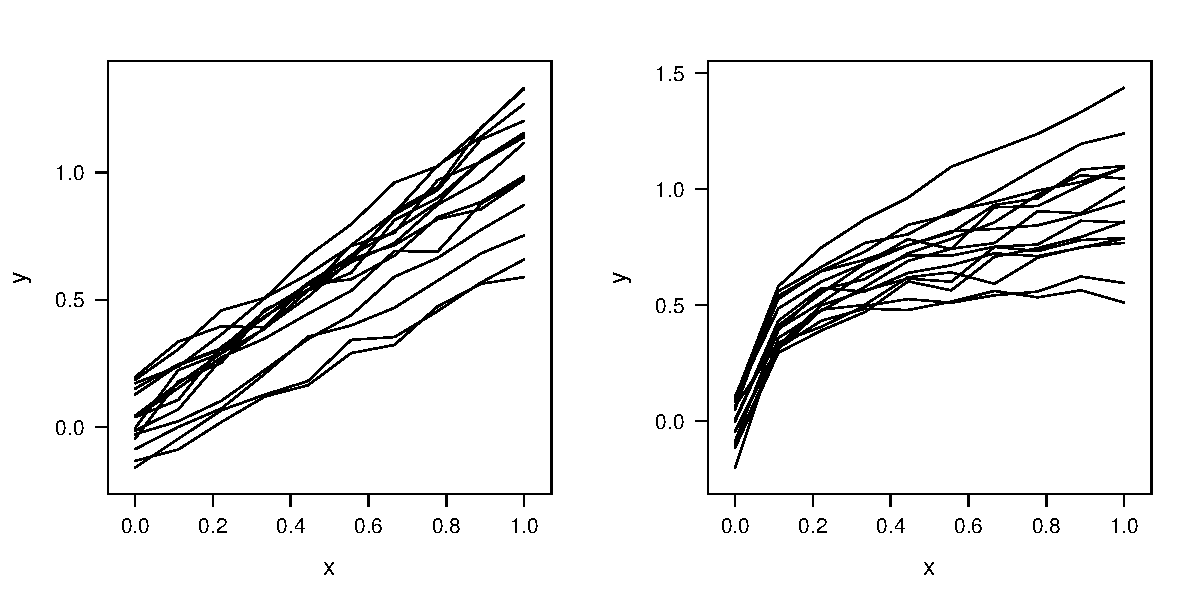
\includegraphics[width=0.8\linewidth]{figure/simulation} 

}

\caption[Spaghetti plots of simulated data]{Spaghetti plots of simulated data. \textit{Left}: Data simulated from Model (1). \textit{Right}: Data simulated from Model (2).\label{fig:simulation}}
\end{figure}


\end{knitrout}


%% Describe the simulation
For each case, we computed $\mathcal{C}_W$, $\mathcal{C}_I$, $\mathcal{C}^\boot_W$, $\mathcal{C}^\boot_I$, and $\mathcal{C}^\boot$ at the $0.95$ level of confidence. The estimated coverage probabilities and lengths are reported in Tables~\ref{tab:results-1} and \ref{tab:results-2}. %An extended version of each table that additionally reports the estimated standard error of the length is provided in Web Appendix B. 
The standard deviation of the coverage estimates is approximately $\sqrt{0.95\left(1-0.95\right)/1000} = 0.007$. 

%% Summarize the results
We see from the Table~\ref{tab:results-1} that the coverage is fairly close to the nominal level of 0.95 for all five methods, though there is a slight problem with under-coverage at larger values $x_0$ where the variation in the response is highest. The average lengths of the intervals is also comparable across all five methods. From Table~\ref{tab:results-2}, we see that the Wald intervals $\mathcal{C}_W$ and $\mathcal{C}^\boot_W$ performed rather poorly with respect to coverage when compared to the inversion and percentile bootstrap intervals as $x_0$ is increased, though the coverage for all five intervals decreased for large values of $x_0$ (as expected). These results indicate to us that it is safest to use the inversion and percentile bootstrap intervals when there is curvature in the population mean response. Even when all the intervals perform similarly --- as in Table~\ref{tab:results-1} --- the parametric bootstrap procedure provides an estimate of the entire sampling distribution of $\widehat{x}_0$, rather than just a standard error and confidence interval for $x_0$. And while the inversion and bootstrap adjusted inversion intervals seem to perform well, they may not always produce a finite interval, such is the case for $\mathcal{C}_I$ and $\mathcal{C}^\boot_I$ in the last four columns of Table~\ref{tab:results-2}. The percentile interval, on the other hand, always exists as long as the point estimate exists (i.e., when the population mean response is monotonic in the region of interest).

%% Other comments about the simulation
Although we favor the percentile interval ($\mathcal{C}^\boot$), there are many other types of bootstrap confidence intervals that may be worth considering; see for example, \citet[chap. 5]{davison_bootstrap_1997}. Bootstrap confidence intervals are typically calculated using as large a bootstrap sample size as possible. However, due to limited time and computational power, the number of bootstrap samples used in this simulation was $R = 999$. While this is a modest number to use, we suspect that the coverage of the parametric bootstrap intervals may improve, albeit only slightly, if $R$ was on the order of 9,999 or so. Secondly, a number of other important factors were held fixed in this study (e.g., the sample sizes and variance components). To investigate how these parameters affect the length and coverage estimates of the intervals under question, a much larger Monte Carlo study is required. 

\begin{table}[!htb]
\centering
\caption{Coverage and length of 95\% confidence intervals for data generated by Model 1. \label{tab:results-1}}
\begin{tabular}{llcccccc}
  \toprule
            &  $x_0 =$               & 0    & 0.25 & 0.5  & 0.75 & 1 \\
  \hline
  Coverage  &  $\mathcal{C}_W$       & 0.97 & 0.95 & 0.93 & 0.93 & 0.92 \\
            &  $\mathcal{C}_I$       & 0.95 & 0.95 & 0.93 & 0.92 & 0.92 \\
            &  $\mathcal{C}^\star_W$ & 0.97 & 0.95 & 0.93 & 0.91 & 0.92 \\
            &  $\mathcal{C}^\star_I$ & 0.97 & 0.96 & 0.94 & 0.92 & 0.92 \\
            &  $\mathcal{C}^\star$   & 0.96 & 0.95 & 0.93 & 0.92 & 0.93 \\
  \hline
  Length    &  $\mathcal{C}_W$       & 0.43 & 0.49 & 0.62 & 0.80 & 1.00 \\
            &  $\mathcal{C}_I$       & 0.44 & 0.49 & 0.63 & 0.81 & 1.02 \\
            &  $\mathcal{C}^\star_W$ & 0.43 & 0.49 & 0.62 & 0.81 & 1.02 \\
            &  $\mathcal{C}^\star_I$ & 0.46 & 0.51 & 0.65 & 0.85 & 1.08 \\
            &  $\mathcal{C}^\star$   & 0.44 & 0.49 & 0.63 & 0.81 & 1.02 \\
  \bottomrule
\end{tabular}\vskip18pt
\end{table}

\begin{table}[!htb]
\centering
\caption{Coverage and length of 95\% confidence intervals for data generated by Model 2. An average length of $\infty$ indicates that the upper confidence limit was positive infinite. \label{tab:results-2}}
\begin{tabular}{llcccccc}
  \toprule
            &  $x_0 =$               & 0    & 0.25 & 0.5  & 0.75 & 1 \\
  \hline
  Coverage  &  $\mathcal{C}_W$       & 1.00 & 0.91 & 0.89 & 0.85 & 0.83 \\
            &  $\mathcal{C}_I$       & 0.94 & 0.96 & 0.92 & 0.90 & 0.87 \\
            &  $\mathcal{C}^\star_W$ & 1.00 & 0.89 & 0.88 & 0.88 & 0.84 \\
            &  $\mathcal{C}^\star_I$ & 0.94 & 0.96 & 0.93 & 0.93 & 0.90 \\
            &  $\mathcal{C}^\star$   & 0.95 & 0.95 & 0.93 & 0.93 & 0.90 \\
  \hline
  Length    &  $\mathcal{C}_W$       & 0.02 & 0.64 & 1.34 & 2.39 & 4.46 \\
            &  $\mathcal{C}_I$       & 0.05 & $\infty$ & $\infty$ & $\infty$ & $\infty$ \\
            &  $\mathcal{C}^\star_W$ & 0.05 & 1.13 & 3.33 & 5.75 & 7.20 \\
            &  $\mathcal{C}^\star_I$ & 0.05 & $\infty$ & $\infty$ & $\infty$ & $\infty$ \\
            &  $\mathcal{C}^\star$   & 0.05 & 0.70 & 2.04 & 4.18 & 5.66\\
  \bottomrule
\end{tabular}\vskip18pt
\end{table}

\section{Bladder Volume Data}
\label{sec:bladder}
In this section, we illustrate the techniques described in the previous section on a real dataset taken from \citet{brown_measurement_1993}. In Brown's words
\begin{quotation}
\noindent"A series of 23 women patients attending a urodynamic clinic were recruited for the study. After successful voiding of the bladder, sterile water was introduced in additions of 10, 15, and then 25 ml increments up to a final cumulative total of 175 ml. At each volume a measure of height ($\texttt{H}$) in mm and depth ($\texttt{D}$) in mm of largest ultrasound bladder images were taken. The product $\texttt{H} \times \texttt{D}$ was taken as a measure of liquid volume...
"\end{quotation}
The product of $\code{H}$ and $\code{D}$ is plotted against true volume in Figure~\ref{fig:bladder-spaghetti} for each of the 23 subjects. As can be seen from this plot, each subject has a slightly nonlinear trend and there are some missing observations (i.e., the data are unbalanced). Both \citet{brown_measurement_1993} and \citet{oman_calibration_1998} suggested transforming the data first. For instance, a simple \textit{log-log} transformation produces a relatively linear trend for each subject. However, not all data can be transformed as successfully, thus, we will leave the data on the original scale and simply model the nonlinearity with a quadratic term. Let $\code{HD}_{ij}$ be the $j$-th measurement for the $i$-th subject. The model we use is a second-degree polynomial with uncorrelated random effects for the intercept and linear terms:
\[
  \code{HD}_{ij} = \beta_0+\mathscr{B}_{0i} + \left(\beta_1+\mathscr{B}_{1i}\right)\code{volume}_{ij} + \beta_3\code{volume}_{ij}^2 + \epsilon_{ij},
\]
where $\mathscr{B}_{0i} \sim \mathcal{N}\left(0, \tau_0^2\right)$ independent of $\mathscr{B}_{1i} \sim \mathcal{N}\left(0, \tau_1^2\right)$ and $\epsilon_{ij} \sim \mathcal{N}\left(0, \sigma_\epsilon^2\right)$.

\begin{knitrout}
\definecolor{shadecolor}{rgb}{0.969, 0.969, 0.969}\color{fgcolor}\begin{figure}[]


{\centering 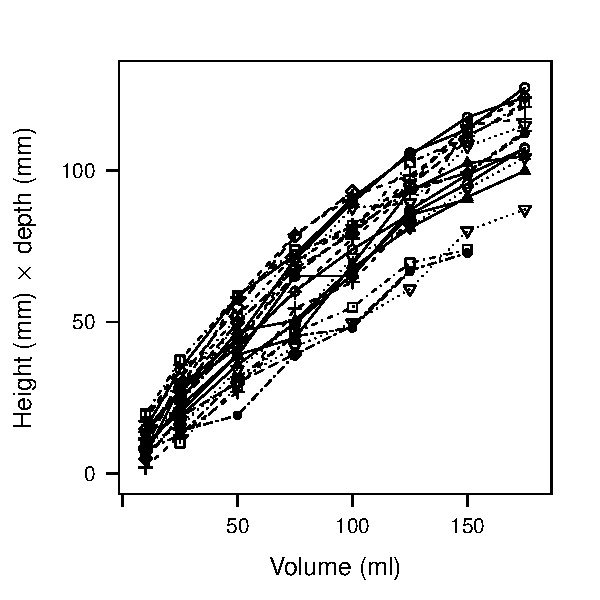
\includegraphics[width=0.8\linewidth]{figure/bladder-spaghetti} 

}

\caption[Scatterplot of the bladder volume data]{Scatterplot of the bladder volume data. Lines connect measurements belonging to the same person.\label{fig:bladder-spaghetti}}
\end{figure}


\end{knitrout}


Suppose we obtain a new observation, $\code{HD}_0 = 85 \text{ mm}^2$, for which the true volume is unknown. To estimate the unknown volume, denoted $v_0$, we solve the equation 
\[
  \widehat{\mu}\left(v_0\right) = \widehat{\beta}_0 + \widehat{\beta}_1v_0 + \widehat{\beta}_2v_0^2 = 85 \text{ mm}^2
\]
for $v_0$ using the quadratic formula. The point estimate obtained is $\widehat{v}_0 = 120.5289$ ml (see Figure~\ref{fig:histogram}). The corresponding R code is given an R Example 2 in Web Appendix B.




R Example 3 from Web Appendix B shows how to use the \proglang{R} package \pkg{car} to compute the approximate standard error based on the first-order Taylor series estimate given in Equation~\eqref{eqn:cal-lmm-approx}. Note that our model has $\var\left[\mathscr{Y}_0\right] = \tau_0^2 + x_0^2\tau_1^2 + \sigma_\epsilon^2$ where $\tau_0^2$ and $\tau_1^2$ are the variances of the random intercept and linear term, respectively. The estimated standard error of $\widehat{v}_0$ is 26.1981 which yields an approximate 95\% Wald-based confidence interval for $v_0$ of $(69.1815, 171.8763)$.

Obtaining the inversion interval \eqref{eqn:inversion} is less straightforward; in \proglang{R}, we have to write our own prediction function that will return the standard errors of the fitted values. R Example 4 from Web Appendix B shows the minimal \proglang{R} code necessary to obtain $\mathcal{C}_I$ for the bladder volume example. The resulting interval, $(75.3908, 184.7025)$, is only slightly larger than the Wald interval. Notice the inversion interval is not symmetric about the inverse estimate $\widehat{v}_0 = 120.5289 \text{ ml}$ which, given the nonlinear trend and increasing variation in the data, is more realistic. In addition, we may also obtain the bootstrap adjusted inversion interval \eqref{eqn:inversion-boot} described in Section~\ref{sec:inversion-adjusted} --- see R example 5 in Web Appendix B which uses the new \code{bootMer} function in the \proglang{R} package \pkg{lme4} to perform the parametric bootstraps outlined in Section~\ref{sec:parametric}.. A histogram of the 9,999 bootstrap replicates of the predictive pivot $\mathcal{Q}$ is also given in the appendix. The estimated sampling distribution of $\mathcal{Q}$ seems reasonably normal. The necessary quantiles to compute $\mathcal{C}^\boot_I$ are $q^\boot_{0.025} = -2.0031$ and $q^\boot_{0.975} = 1.9804$ (comparable to the corresponding quantiles from a standard normal distribution; i.e., $\pm 1.96$). Using these quantiles, a 95\% bootstrap adjusted inversion interval for $x_0$ is $\mathcal{C}^\boot_I = (57.94, 138.16)$, which is only slightly wider than the unadjusted inversion interval based on the normal approximation. In short, the normal approximation seems to work quite well for these data. 

Finally, we compute the bootstrap distribution of $\widehat{v}_0$ directly using the algorithm in Figure~\ref{alg:pb} --- see R Example 5 in Web Appendix B. Our results are based on a bootstrap simulation of size $R = 9,999$. Since we do not expect the sampling distribution of $\widehat{v}_0$ to be symmetric, we provide only a 95\% percentile bootstrap interval; that is, the interval obtained by taking the lower 2.5 and upper 97.5 percentiles of the resulting bootstrap distribution. The computed interval, $(58.37, 136.02)$, is quite close to the inversion interval previously obtained. A histogram of $9,999$ bootstrap replicates of $\widehat{v}_0$ is given in Figure~\ref{fig:histogram}. The histogram estimate suggests that the sampling distribution of $\widehat{v}_0$ is positively skewed (the estimated skewness is $0.3011$), providing further support for the inversion and percentile intervals over the symmetric Wald interval. The results for this example are summarized in Table~\ref{tab:results}.

\begin{knitrout}
\definecolor{shadecolor}{rgb}{0.969, 0.969, 0.969}\color{fgcolor}\begin{figure}[]


{\centering 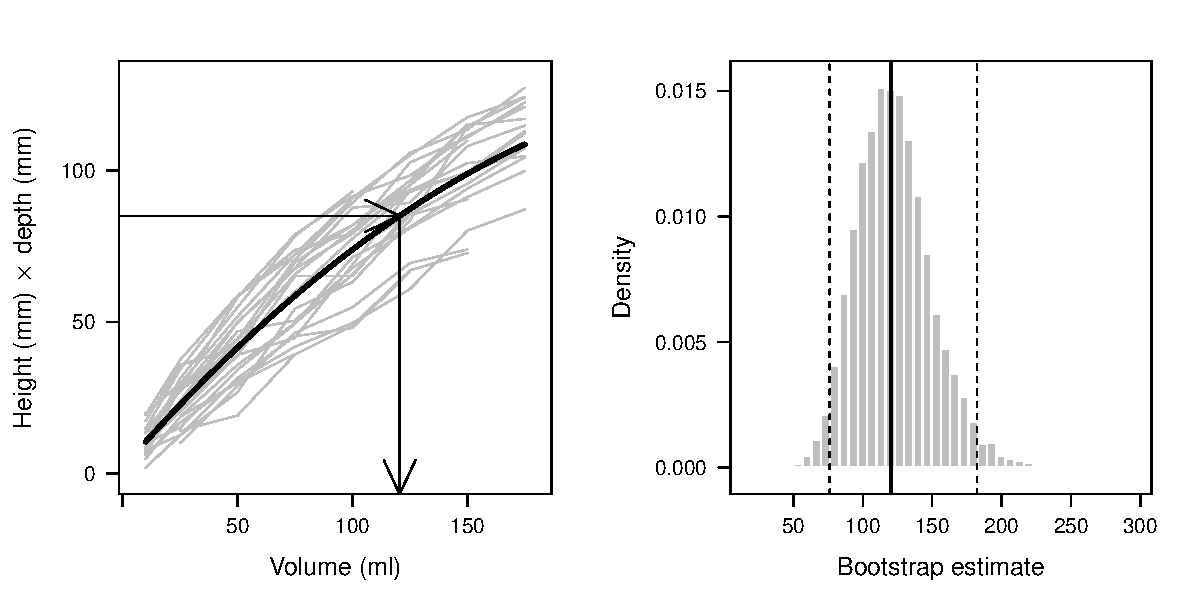
\includegraphics[width=0.8\linewidth]{figure/histogram} 

}

\caption[Bladder data results]{Bladder data results. \textit{Left}: Spaghetti plot of the bladder data with fitted mean response. The horizontal arrow indicates the position of $\code{HD}_0 = 85 \mathrm{\, mm^2}$ and the vertical arrow indicates the position of the inverse estimate, $\widehat{v}_0 = 120.53$ ml. \textit{Right}: Histogram of the 9,999 bootstrap replicates of $\widehat{v}_0$. The solid line indicates the position of the original estimate and the dotted lines represent the sample 0.025 and 0.975 quantiles of the bootstrap distribution of $\widehat{v}_0$.\label{fig:histogram}}
\end{figure}


\end{knitrout}


\begin{table}
\caption{Summary of results for the bladder volume example.}
\label{tab:results}
\begin{center}
\begin{tabular}{lccc}
\toprule %Hline
Interval & \multicolumn{1}{c}{Estimate} &  \multicolumn{1}{c}{SE} & \multicolumn{1}{c}{95\% confidence limits} \\ \hline
$\mathcal{C}_W$       & 120.53 & 26.20 & (69.18, 171.88) \\
$\mathcal{C}_I$       & 120.53 & ---           & (75.39, 184.70) \\
$\mathcal{C}^\boot_W$ & 120.53 & 27.40 & (64.54, 171.96) \\
$\mathcal{C}^\boot_I$ & 120.53 & 27.40 & (74.97, 186.62) \\
$\mathcal{C}^\boot$   & 120.53 & 27.40 & (76.05, 182.24) \\
\bottomrule
\end{tabular}\vskip18pt
\end{center}
\end{table}

\section{Discussion}
\label{sec:discuss}
We have described a number of techniques for controlled calibration in a linear mixed model setting. The Wald interval is the simplest, but relies on the asymptotic normality of $\widehat{x}_0$ along with a Taylor-series approximation of its variance. Perhaps the biggest drawback to using a Wald calibration interval is that it is always symmetric about $\widehat{x}_0$. While this is appealing to many researchers, it is not very realistic in standard situations where, say, the data exhibit nonlinear behavior (e.g., horizontal asymptotes) and nonconstant variance. The asymptotic normality of $\widehat{x}_0$ may also be questioned when it is not the ML estimate, as in the bladder volume example. This is akin to using the Wald method in nonlinear calibration problems (the software JMP does this). The Wald approach may, however, produce reliable inference when the sampling distribution of $\widehat{x}_0$ is reasonably symmetric. Although more difficult to obtain, the inversion interval and its bootstrap adjustment appear more accurate than the Wald intervals, especially when the mean response curve is not linear. However, the inversion interval may not exist for a given observation $y_0$ at the specified confidence level $1-\alpha$. The percentile interval based on the parametric bootstrap algorithm given in this paper is especially promising in that it has comparable coverage probability and length to the inversion intervals; however, unlike the inversion intervals, the percentile parametric bootstrap method will always provides finite confidence limits as long as the fitted population mean response is monotonic in the region of interest. Finally, although we give snippets of \proglang{R} code for implementing the methods described in this paper for the bladder volume data in Web Appendix B, it is likely that a future release of the \proglang{R} package \pkg{investr} \citep{investr_greenwell_2013} will contain this functionality.

%  The \backmatter command formats the subsequent headings so that they
%  are in the journal style.  Please keep this command in your document
%  in this position, right after the final section of the main part of 
%  the paper and right before the Acknowledgements, Supplementary Materials,
%  and References sections. 

\backmatter

%  This section is optional.  Here is where you will want to cite
%  grants, people who helped with the paper, etc.  But keep it short!

\section*{Acknowledgements}

This work was supported by the AFOSR/RTA [grant F1ATA03039J001] \vspace*{-8pt}

%  If your paper refers to supplementary web material, then you MUST
%  include this section!!  See Instructions for Authors at the journal
%  website http://www.biometrics.tibs.org

\section*{Supplementary Materials}

Web Appendices A and B referenced in Sections \ref{sec:est}, \ref{sec:extending}, \ref{sec:parametric}, and \ref{sec:bladder} are available with this paper at the Biometrics website on Wiley Online Library.\vspace*{-8pt}

%  Here, we create the bibliographic entries manually, following the
%  journal style.  If you use this method or use natbib, PLEASE PAY
%  CAREFUL ATTENTION TO THE BIBLIOGRAPHIC STYLE IN A RECENT ISSUE OF
%  THE JOURNAL AND FOLLOW IT!  Failure to follow stylistic conventions
%  just lengthens the time spend copyediting your paper and hence its
%  position in the publication queue should it be accepted.

%  We greatly prefer that you incorporate the references for your
%  article into the body of the article as we have done here 
%  (you can use natbib or not as you choose) than use BiBTeX,
%  so that your article is self-contained in one file.
%  If you do use BiBTeX, please use the .bst file that comes with 
%  the distribution.

\bibliographystyle{biom} \bibliography{lcgd}

\label{lastpage}

\end{document}
